% !TEX root = ../main.tex

\chapter{Concluding Remarks}\label{ch:remarks}
\section{High-Level Contributions and Their Broader Context}
ERC-20 remains the dominant token standard in the Ethereum ecosystem, and resolving longstanding vulnerabilities within its framework is essential for protecting investors. One achievement in this research was addressing the Multiple Withdrawal Attack in 2019, an issue that has persisted since 2016. Following this, our study extended its scope in 2020 to investigate other potential security concerns within ERC-20 implementations. By systematizing 82 distinct vulnerabilities and best practices applicable to ERC-20, the research laid the groundwork for improved token safety. TokenHook, developed in 2021 as part of this work, addresses these vulnerabilities and provides stronger compliance and security compared to the top 10 ERC-20 tokens currently in use.

Beyond technical improvements, this work focused in 2022 on the economic implications of ERC-20's use as a derivative token, particularly within the context of leveraged tokens (LVTs). The analysis identified 10 key shortcomings, ranging from transparency issues to risks associated with market volatility and rebalancing mechanisms. Solutions were proposed for each identified problem, demonstrating the potential for better investor outcomes through targeted improvements.

To understand the landscape further in 2023, the research reviewed six existing decentralized LVTs to evaluate their effectiveness in mitigating these issues. This evaluation revealed gaps in current approaches and underscored the need for a more comprehensive solution. LeverEdge was proposed in 2024 as an hybrid L1-L2 model that (i) inherits the enhanced security properties of TokenHook and (ii) addresses most of the economic and operational deficiencies found in current LVTs. By integrating these advancements, LeverEdge ensures a more secure and reliable investment framework for users.

As shown in Figure \ref{fig:timeline}, the summary of contributions from 2019 to 2024 highlights that, TokenHook directly addresses vulnerabilities inherent in ERC-20 tokens, enhancing security and safeguarding users against potential threats such as the Multiple Withdrawal Attack. LeverEdge, on the other hand, addresses the structural and operational deficiencies found in current leveraged tokens (LVTs), providing a more secure and transparent model for users seeking leveraged exposure to cryptocurrency assets.

\begin{figure}[t]
	\centering
	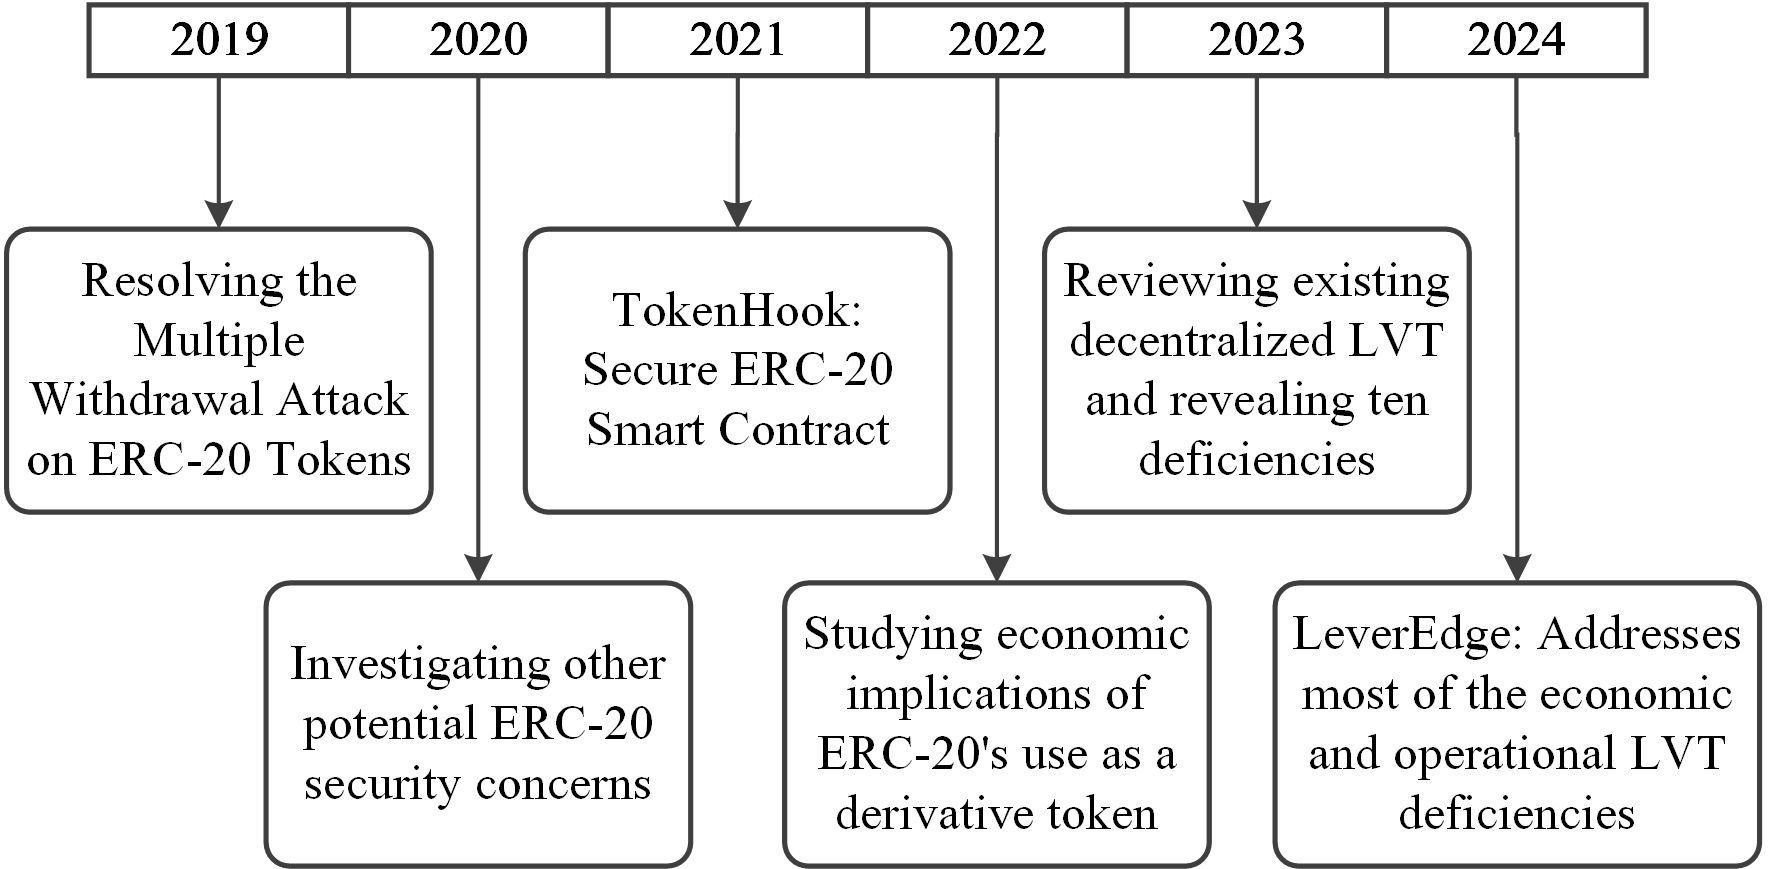
\includegraphics[width=\textwidth,keepaspectratio]{timeline.png}
	\caption[Contributions summary]{Summary of contributions from 2019 to 2024}
	\label{fig:timeline}
\end{figure}

\section{Recommended Changes and Lessons for Ethereum from This Work}
This work is guided by the specific solutions of TokenHook and LeverEdge. It focuses on strengthening investor protection by improving security, user experience, and economic performance within the Ethereum ecosystem. Changes that Ethereum should learn from this work and recommendations are follows.

\subsection{Reform of Approval Mechanisms}
The current \texttt{approve} and \texttt{transferFrom} methods poses risks, particularly through indefinite allowances. To enhance investor protection, the Ethereum ecosystem should consider more secure approval models:

\subsubsection{Session-Based or Single-Use Approvals}
Implementing time-limited or single-use permissions can mitigate the risk of indefinite access. Session-based approvals allow users to grant token allowances for a specific period or session, automatically expiring afterward. Single-use approvals permit a one-time token transfer, after which the allowance is revoked. These mechanisms reduce the risk of unauthorized or forgotten permissions, enhancing overall security.

\subsubsection{ERC-2612 Permit Functionality}
Expanding the use of off-chain approval processes can minimize exposure. ERC-2612~\cite{eip2612} introduces a \texttt{permit} function that enables users to approve token transfers via off-chain signatures, eliminating the need for an on-chain \texttt{approve} transaction. This approach not only reduces gas costs but also enhances security by minimizing the attack surface associated with on-chain approvals.

\subsection{Prioritization of Withdrawal Mechanism Security}
TokenHook's approach to addressing vulnerabilities such as the Multiple Withdrawal Attack highlights the importance of secure withdrawal protocols. Establishing standards for secure withdrawal practices can ensure consistent safety across ERC-20 implementations, reducing investor risk.

\subsection{User-Friendly and Transparent Token Interactions}
Simplifying how users interact with tokens can enhance protection by reducing user error. Recommendations include wallet-level support for contextual allowances and token-level permissions. Integrating clear interfaces and notifications regarding token approvals, their limits, and duration can empower users to make informed decisions and prevent common mistakes such as granting excessive or indefinite permissions. Transparent interaction mechanisms should also include detailed transaction summaries that explain the purpose and consequences of each action, ensuring users know exactly how their tokens are being utilized. 

\section{Future Work}
The findings of this research underscore the critical importance of investor protection within the Ethereum ecosystem, achieved through targeted solutions addressing specific vulnerabilities and deficiencies in token standards. The development of TokenHook and LeverEdge exemplifies how focused improvements can enhance the safety and reliability of decentralized finance (DeFi) interactions. But still work on the following in the future can create more resilient, transparent, and user-friendly instruments align with investor expectations and the evolving DeFi landscape.

\subsection{Enhancing the Security of Other Fungible Tokens}
Future research on ERC-20 tokens should broaden its focus to include other types of fungible tokens, including, but is not limited to, the exploration of ERC-777 and ERC-1155 tokens.

\subsection{Improved Rebalancing Algorithms}
One of the primary issues with LVTs is the volatility decay resulting from frequent rebalancing. Future research could explore more efficient and adaptive rebalancing algorithms that minimize value erosion, especially in high-volatility markets. Machine learning techniques could be applied to predict optimal rebalancing times, reducing the negative impact of market swings on leveraged positions

\subsection{Cross-Chain Leveraged Tokens}
Future work could investigate creating LVTs that function seamlessly across multiple blockchain ecosystems. Cross-chain capabilities could improve access to different DeFi platforms and liquidity pools, enhancing the usability and adoption of LVTs while reducing exposure to a single network's limitations or issues.

\subsection{Leveraging Account Abstraction (AA) for Enhanced User Protection}
Account abstraction (AA) has the potential to significantly improve user protection by allowing transactions to be bundled and executed under user-defined conditions~\cite{Ethereum_AA}. It can integrate security checks directly into wallet operations. This makes it possible for users to implement tailored permissions and rules for token interactions, adding an extra layer of protection on top of the built-in safeguards of the TokenHook and LeverEdge. While AA complements the work done on the token contract level, future research could explore how AA can be used to create safer, user-controlled mechanisms for rebalancing or stopping trades based on pre-set criteria.